In this chapter, we present a comprehensive look at the Hungarian algorithm. The algorithm relies on 
some interesting techniques, which we spell out carefully. Ultimately, we show how this algorithm 
solves its associated primal and dual linear programs -- the maximum weight matching and 
the minimum weight vertex cover problems, respectively.

\begin{section}{Preliminaries}
	In this section, we use the motivation of the linear programs to develop an algorithm for 
	simultaneously solving the maximum weight matching and minimum weight vertex cover problems. 
	Our algorithm works by taking every exposed vertex on the left, and from each such 
	vertex building a collection of alternating paths. For our graphs $G = (U,V,E)$ we will assume 
	$|U| = |V|$.
	
	Let us remind ourselves what the primal-dual linear programs
	motivate. We want to minimize $\sum w_{uv}$ and maximize $(\sum_u y_u + \sum_v y_v)$. Moreover, 
	we want optimal solutions (i.e. $\sum w_{uv} = \sum_u y_u + \sum_v y_v$). For our primal, we are 
	keeping track of edge weights. For the dual, we will be keeping track of a ``labeling'' on 
	vertices, given by the $y_u$ and $y_v$ values. We define what a labeling is now.
	\begin{definition}
		A \emph{vertex labeling} on a weighted bipartite graph $G = (U,V,E)$ is a function 
		$l: U\cup V \to \N$. We call a labeling \emph{feasible} if for all $u\in U$ and 
		$v\in V$, $l(u) + l(v) \geq w_{uv}$.
	\end{definition}
	This labeling corresponds to our dual variables; a feasible labeling is a feasible dual 
	solution. It will be helpful for us to look at a certain subset of our graph where the labeling 
	is exact (i.e. where $l(u) + l(v) - w_{uv} = 0$).
	\begin{definition}
		The \emph{equality subgraph} of $G = (U,V,E)$ is the graph $G_l = (U,V,E_l)$, 
		where 
		\[
			E_l = \{(u,v)\ :\ l(u) + l(v) = w_{uv}\}.
		\]
	\end{definition}
	In Figure 3.1 we show a bipartite graph along with its corresponding equality graph.
	\begin{figure}[h]
		\centering
		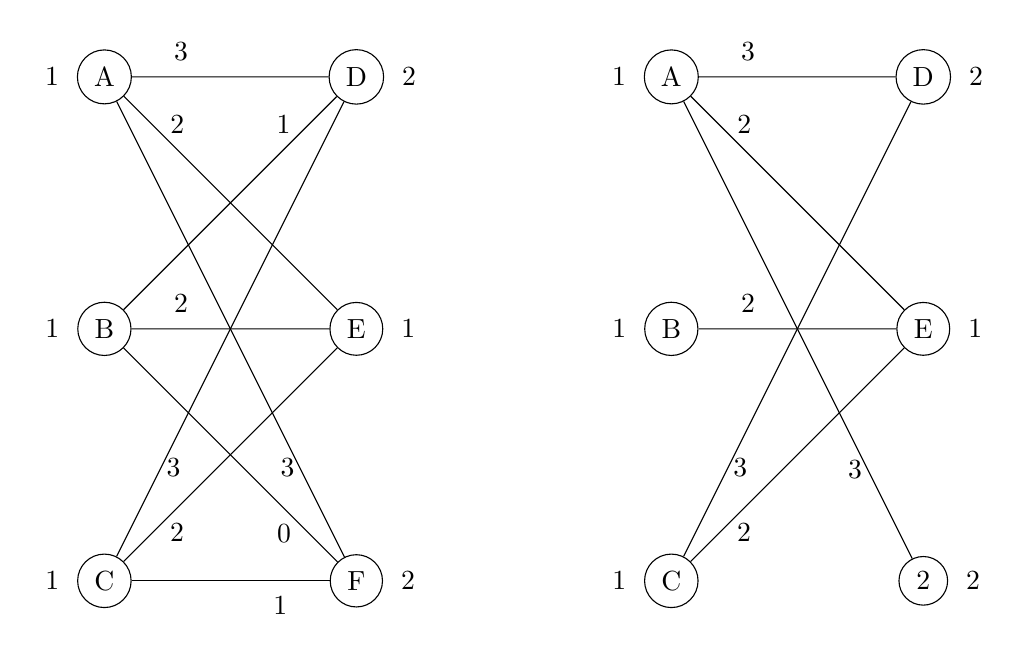
\begin{tikzpicture}[scale=.8,auto=left,every node/.style={circle,draw=black}]
			%left nodes
			\node [label=left:{1}] (n1) at (1,10) {A};
			\node [label=left:{1}] (n2) at (1,6) {B};
			\node [label=left:{1}] (n3) at (1,2) {C};

			%right nodes
			\node [label=right:{2}] (n4) at (5,10) {D};
			\node [label=right:{1}] (n5) at (5,6) {E};
			\node [label=right:{2}] (n6) at (5,2) {F};

			%edges
			\draw (n1) -- node[near start,draw=none,above] {3} ++(n4);
			\draw (n1) -- node[near start,draw=none,above] {2} ++(n5);
			\draw (n1) -- node[near end,draw=none,below] {3} ++(n6);

			\draw (n2) -- node[near end,draw=none,above] {1} ++(n4);
			\draw (n2) -- node[near start,draw=none,above] {2} ++(n5);
			\draw (n2) -- node[near end,draw=none,below] {0} ++(n6);

			\draw (n3) -- node[near start,draw=none,below] {3} ++(n4);
			\draw (n3) -- node[near start,draw=none,below] {2} ++(n5);
			\draw (n3) -- node[near end,draw=none,below] {1} ++(n6);


			%left nodes
			\node [label=left:{1}] (n7) at (10,10) {A};
			\node [label=left:{1}] (n8) at (10,6) {B};
			\node [label=left:{1}] (n9) at (10,2) {C};

			%right nodes
			\node [label=right:{2}] (n10) at (14,10) {D};
			\node [label=right:{1}] (n11) at (14,6) {E};
			\node [label=right:{2}] (n12) at (14,2) {2};

			%edges
			\draw (n7) -- node[near start,draw=none,above] {3} ++(n10);
			\draw (n7) -- node[near start,draw=none,above] {2} ++(n11);
			\draw (n7) -- node[near end,draw=none,below] {3} ++(n12);

			\draw (n8) -- node[near start,draw=none,above] {2} ++(n11);

			\draw (n9) -- node[near start,draw=none,below] {3} ++(n10);
			\draw (n9) -- node[near start,draw=none,below] {2} ++(n11);
		\end{tikzpicture}
		\caption{A weighted bipartite graph (left) and its corresponding equality subgraph
		(right).}
	\end{figure}
	\begin{theorem}{(Kuhn-Munkres)}
		If $l$ is a feasible labeling and $M$ is a perfect matching in $G_l$ then $M$ is a 
		maximum weight matching.
	\end{theorem}

	\begin{proof}
		Let $M\'$ be a perfect matching in $G$. Since every $u\in U\cup V$ is included 
		in exactly one edge in $M\'$, then 
		\[
			\sum_{(u,v)\in M\'} w_{uv} \leq \sum_{(u,v)\in M\'} (l(u)+l(v)) = 
			\sum_{z\in U\cup V} l(z).
		\]
		This says that the sum of our label values is an upper bound on the weight of any 
		perfect matching.

		Now suppose that $M$ is a perfect matching in $G_l$. Then 
		\[
			\sum_{(u,v)\in M} w_{uv} = \sum_{z\in U\cup V} l(z).
		\]
		So $\sum_{(u,v)\in M\'} w_{uv} \leq \sum_{(u,v)\in M} w_{uv}$, 
		meaning that $M$ must be a maximum weight matching.
	\end{proof}
	
	This theorem tells us that if we can give an algorithm for finding a perfect matching in the 
	equality subgraph (if such a matching exists), then we can find a maximum weight matching in the 
	graph. To do this, we will first define a few terms. 

	As in Chapter 2, let $R$ be the set of vertices reachable from unmatched vertices in $U$ via 
	alternating paths, 
	and let $S:=R\cap U$, $T:=R\cap V$. We will use these sets to construct our collection of 
	alternating trees as defined in Chapter 2. Let $M$ be our maximum cardinality matching.
	
	Now, consider a feasible labeling $l$ on a graph $G = (U,V,E)$ and set 
	\[
		\delta := \min_{u\in S,\ v\notin T} \{l(u) + l(v) - w_{uv} \}.
	\]
	We define a new labeling $l^{'}$ as follows:
		\[
			l\' (z) = 
			\begin{cases}
				l(z) - \delta &\text{ if } z\in S \\
				l(z) + \delta &\text{ if } z\in T \\
				l(z) &\text{ otherwise.}
			\end{cases}
		\]
	\begin{lemma}
		The labeling $l^{'}$ as defined above is a feasible labeling.
	\end{lemma}

	\begin{proof}
		To show this labeling is feasible, we must show that for any edge $(u,v)$, 
		$l^{'}(u) + l^{'}(v) \geq w_{uv}$. For $u\in U$, $v\in V$, there are four possibilities:
		\begin{enumerate}
			\item If $u\in S$ and $v\in T$ then $l\' (u) + l\' (v) = l(u) + l(v)$. This 
				is because $l^{'}(u) = l(u) - \delta$ and $l^{'}(v) = l(v) + \delta$. 
			\item If $u\notin S$ and $v\notin T$, $l\' (u) = l(u)$ and $l\' (v) = l(v)$, 
				so $l\' (u) + l\' (v) = l(u) + l(v)$.
			\item If $u\in S$ and $v\notin T$, $l\' (u)=l(u) - \delta$ and $l\' (v) = l(v)$. 
				We know $\delta = \min_{u\in S,v\notin T} \{l(u) + l(v) - w_{uv}\}$, 
				which means $\delta \leq l(u) + l(v) - w_{uv}$, and thus 
				$l\' (u) + l\' (v) \geq w_{uv}$.
			\item If $u\notin S$ and $v\in T$, $l\' (u) = l(u)$ and $l\' (v) = l(v) + 
				\delta$. So we get $l^{'}(u) + l^{'}(v) = l(u) + l(v) + \delta \geq 
				w_{uv}$.
		\end{enumerate}
	\end{proof}
	We also need to show that this labeling increases the size of our equality graph.
	\begin{lemma}
		Given an initial feasible labeling $l$ and the labeling $l^{'}$, the following 
		hold:
		\begin{enumerate}
			\item If $(u,v)\in E_l$ and $u\in S$, $v\in T$, then $(u,v)\in E_{l^{'}}$. 
			\item If $(u,v)\in E_l$ and $u\notin S$, $v\notin T$, then $(u,v)\in 
				E_{l^{'}}$.
			\item If $u\notin S$ and $v\in T$, then $(u,v)\notin E_l$.
			\item If $u\in S$ and $v\notin T$ then $(u,v)\notin E_l$.
			\item There exists some $(u,v)$ such that $u\in S$ and $v\notin T$, and 
				$(u,v)\in E_{l^{'}}$. 
		\end{enumerate}
	\end{lemma}
	\begin{proof}
		The claims (1) and (2) are made clear by the previous lemma. \\
		To prove claim (3), suppose towards a contradiction that $(u,v)\in E_l$ with 
		$u\notin S$ and $v\in T$. This means that since $v\in T$, $u$ is reachable by some 
		alternating path in $R$, hence $u\in S$, which is a contradiction.\\
		Part (4) follows from the fact that if $u\in S$ and $(u,v)\in E_l$, then $v$ is 
		reachable by an alternating path in $R$, hence $v\in T$, which is a contradiction.\\
		To see (5), note that there is some edge $(u,v)$ with 
		$u\in S$, $v\notin T$ such that $\delta = l(u) + l(v) - w_{uv}$, so when we take 
		$l\' (u) = l(u) - \delta$ and $l\' (v) = l(v)$, we get 
		\begin{align*}
			l\' (u) + l\' (v) - w_{uv} &= l(u) - \delta + l(v) - w_{uv} \\
						   &= l(u) + l(v) - w_{uv} - \delta \\
						   &= \delta - \delta \\
						   &= 0.
		\end{align*}
		This is exactly what it means for an edge $(u,v)$ to be in $E_l$. Hence $E_l \subset 
		E_{l^{'}}$. 
	\end{proof}

	\begin{theorem}
		$|E_l| < |E_{l^{'}}|$.
	\end{theorem}

	The proof of this theorem follows from the previous lemma, as we showed that 
	$E_l \subset E_{l^{'}}$.
\end{section}
\begin{section}{The Hungarian Algorithm}
	We now look at the Hungarian method for finding maximum-weight matchings on bipartite graphs. 
	This method was originally developed by Kuhn and Munkres, who named it in honor of the Hungarian 
	mathematicians K\H{o}nig and Egervary. The algorithm is shown in Figure 3.2.
	\begin{figure}[h]
	\begin{center}
		\begin{minipage}{3in}
			\begin{codebox}
				\Procname{$\proc{Hungarian-Max-Assign} (U,V,E,w)$}
				\li $l_u := \max_{v} c_{uv}$
				\li $l_v := 0$
				\li Repeatedly do:
				\li \quad $M := $ $\proc{Max-Card-Matching} (U,V,G_l)$
				\li \quad \If $M$ is a perfect matching in $G_l$
				\li \quad	\Then 
				    \quad		\Return $M$
				    \quad	\End
				\li \quad $R := $ $\proc{Alt-Path-Reachable} (U,V,E_l,M)$
				\li \quad $l :=$ $\proc{Label-Update} (R,U,V,E,w,l)$
			\end{codebox}
		\end{minipage}
	\end{center}
		\caption{The Hungarian Algorithm}
	\end{figure}
	The correctness of the algorithm follows from the lemma and theorem. Note that our labeling $l$ 
	remains feasible by Lemma 3.4, and the equality graph increases in size by Lemma 3.5. This tells 
	us that, assuming our graph $G$ has a perfect matching, one will eventually be found by this 
	algorithm. Since this perfect matching will be in $G_l$, Theorem 3.3 tells us that our final 
	matching $M$ will be of maximum weight.

	We now provide an example of this algorithm. This example is due to Golin \cite{hknotes}.
	\begin{figure}[h]
		\centering
		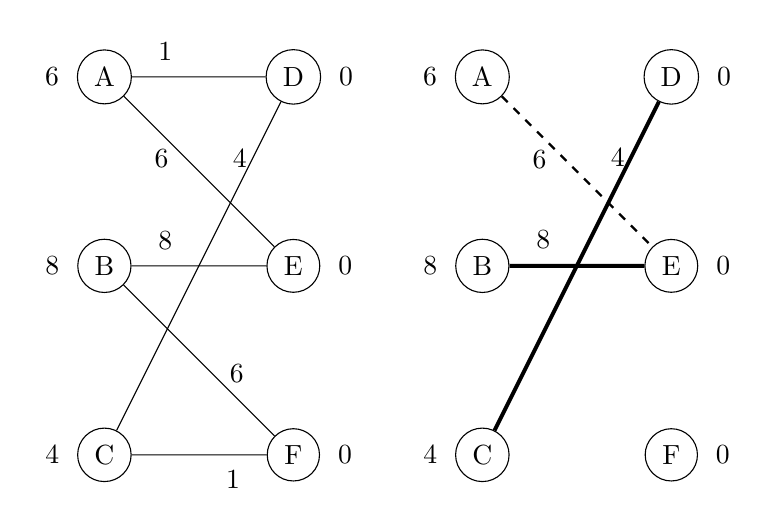
\begin{tikzpicture}[scale=.8,auto=left,every node/.style={circle,draw=black}]

			%left nodes
			\node [label=left:{6}] (n1) at (1,10) {A};
			\node [label=left:{8}] (n2) at (1,7) {B};
			\node [label=left:{4}] (n3) at (1,4) {C};

			%right nodes
			\node [label=right:{0}] (n4) at (4,10) {D};
			\node [label=right:{0}] (n5) at (4,7) {E};
			\node [label=right:{0}] (n6) at (4,4) {F};

			%edges
			\draw (n1) -- node[near start, draw=none, above] {1} ++ (n4);
			\draw (n1) -- node[near start, draw=none, below] {6} ++ (n5);
			\draw (n2) -- node[near start, draw=none, above] {8} ++ (n5);
			\draw (n2) -- node[near end, draw=none, above] {6} ++ (n6);
			\draw (n3) -- node[near end, draw=none, above] {4} ++ (n4);
			\draw (n3) -- node[near end, draw=none, below] {1} ++ (n6);

			
			
			%left nodes
			\node [label=left:{6}] (m1) at (7,10) {A};
			\node [label=left:{8}] (m2) at (7,7) {B};
			\node [label=left:{4}] (m3) at (7,4) {C};

			%right nodes
			\node [label=right:{0}] (m4) at (10,10) {D};
			\node [label=right:{0}] (m5) at (10,7) {E};
			\node [label=right:{0}] (m6) at (10,4) {F};
			
			%edges
			\draw[thick,dashed] (m1) -- node[near start, draw=none, below] {6} ++ (m5);
			\draw[line width=0.5mm] (m2) -- node[near start, draw=none, above] {8} ++ (m5);
			\draw[line width=0.5mm] (m3) -- node[near end, draw=none, above] {4} ++ (m4);
		\end{tikzpicture}
		\caption{Bipartite graph (left) and corresponding equality graph (right) with initial 
		matching}
	\end{figure}
	Our initial matching is $M = \{(\mbox{B},\mbox{E}), (\mbox{C},\mbox{D})\}$ (see Figure 3.3). 
	Note that the current state of 
	the graph is 
	primal-dual feasible. This matching $M$ is not perfect in $G_l$. The unmatched vertices in $U$ 
	consists of a single member, $\mbox{A}$, meaning our algorithm chooses $\mbox{A}$ to add to $R$. 
	So we have 
	$S=\{\mbox{A}\}$ and $T=\{\mbox{E}\}$ since $\mbox{E}$ is reaches to $\mbox{A}$ via the single 
	path. The vertex $\mbox{E}$ is matched, so we grow our alternating tree as follows: 
	$R := R\cup \{\mbox{B}\} = \{\mbox{A},\mbox{B}\}$, 
	$T := T\cup \{\mbox{E}\} = \{\mbox{E}\}$. At this point we adjust our labeling.
	Calculate $\delta = \min _{u\in S,v\notin T} \{l(u) + l(v) - w_{uv}\} = 2$ from edge 
	$(\mbox{B},\mbox{F})$. 
	Our new equality graph is shown in Figure 3.4.
	\begin{figure}[H]
		\centering
		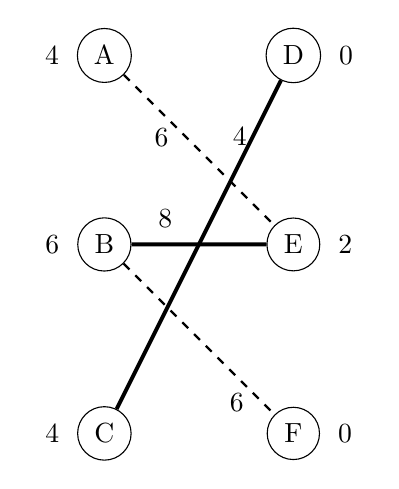
\begin{tikzpicture}[scale=.8,auto=left,every node/.style={circle,draw=black}]
			%left nodes
			\node [label=left:{4}] (m1) at (7,10) {A};
			\node [label=left:{6}] (m2) at (7,7) {B};
			\node [label=left:{4}] (m3) at (7,4) {C};

			%right nodes
			\node [label=right:{0}] (m4) at (10,10) {D};
			\node [label=right:{2}] (m5) at (10,7) {E};
			\node [label=right:{0}] (m6) at (10,4) {F};
			
			%edges
			\draw[thick,dashed] (m1) -- node[near start, draw=none, below] {6} ++ (m5);
			\draw[line width=0.5mm] (m2) -- node[near start, draw=none, above] {8} ++ (m5);
			\draw[thick,dashed] (m2) -- node[near end, draw=none, below] {6} ++ (m6);
			\draw[line width=0.5mm] (m3) -- node[near end, draw=none, above] {4} ++ (m4);
		\end{tikzpicture}
		\caption{Second equality graph.}
	\end{figure}
	Now, $S = \{\mbox{A},\mbox{B}\}$ is the same, but $T = \{\mbox{E},\mbox{F}\}$ has changed (we've 
	implicitly updated $R$). 
	The vertex $F$ is unmatched, meaning it is 
	an endpoint of an augmenting path. In particular, $p = \mbox{A}\to \mbox{E}\to \mbox{B}\to 
	\mbox{F}$ is an augmenting path. Thus we can 
	improve our matching with $M := M\oplus p = \{(\mbox{A},\mbox{E}), (\mbox{B},\mbox{F}), 
	(\mbox{C},\mbox{D})\}$. Our equality graph with 
	the new matching is given in Figure 3.5.
	\begin{figure}[H]
		\centering
		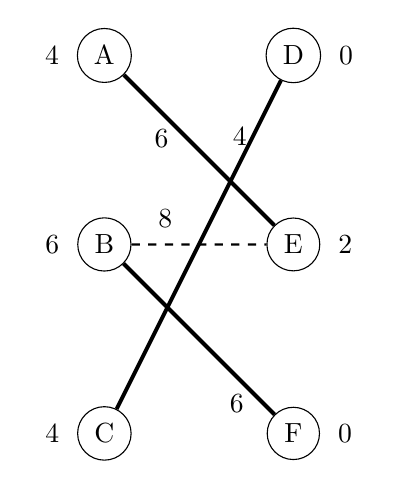
\begin{tikzpicture}[scale=.8,auto=left,every node/.style={circle,draw=black}]
			%left nodes
			\node [label=left:{4}] (m1) at (7,10) {A};
			\node [label=left:{6}] (m2) at (7,7) {B};
			\node [label=left:{4}] (m3) at (7,4) {C};

			%right nodes
			\node [label=right:{0}] (m4) at (10,10) {D};
			\node [label=right:{2}] (m5) at (10,7) {E};
			\node [label=right:{0}] (m6) at (10,4) {F};
			
			%edges
			\draw[line width=0.5mm] (m1) -- node[near start, draw=none, below] {6} ++ (m5);
			\draw[thick,dashed] (m2) -- node[near start, draw=none, above] {8} ++ (m5);
			\draw[line width=0.5mm] (m2) -- node[near end, draw=none, below] {6} ++ (m6);
			\draw[line width=0.5mm] (m3) -- node[near end, draw=none, above] {4} ++ (m4);
		\end{tikzpicture}
		\caption{Equality graph after augmenting.}
	\end{figure}
	This is a perfect matching on the equality graph, so this matching must be a maximum weight 
	matching on the graph. We can check that the values of the primal and dual solutions agree. 
	The sum of weights in the matching is $6+6+4 = 16$, and the sum of the values of our 
	dual variables is $4+6+4+2 = 16$.

	Note that if we want to just find a maximum cardinality matching on a bipartite graph, 
	we can just give all edges weight one and run this algorithm.

	This algorithm was one of the first primal-dual algorithms developed, and it anticipated many 
	later variations on the same theme. It displays the surprising connection between combinatorial 
	optimization and linear programming, which we explore in the next section.
\end{section}
